\documentclass[a4paper,11pt]{article}
%\documentclass[a4paper,11pt]{scrartcl}

\usepackage[a4paper,bindingoffset=0.2in,%
            left=1in,right=1in,top=1in,bottom=1in,%
            footskip=.25in]{geometry}
\usepackage[utf8]{inputenc}
\usepackage{listings}
\usepackage{color}
\usepackage[pdftex,pdfpagelabels,bookmarks,hyperindex,hyperfigures]{hyperref}
\hypersetup{
    bookmarksnumbered=true,     
    bookmarksopen=true,         
    bookmarksopenlevel=1,       
    colorlinks=true,
    allcolors=blue,
    pdfstartview=Fit,           
    pdfpagemode=UseOutlines
}
\usepackage{hypcap}
\usepackage{url}
\usepackage{graphicx}
\renewcommand{\familydefault}{\sfdefault}

\definecolor{mygray}{gray}{0.95}

\lstset{ 
  basicstyle=\footnotesize\ttfamily,        % the size of the fonts that are used for the code
  backgroundcolor=\color{mygray},
  language=Python,
  keywordstyle=\color{blue},
  stringstyle=\color{red},
  commentstyle=\color{cyan},
  keepspaces=true,
  columns=flexible,
  tabsize=1,
  showstringspaces=false
}

\title{Introduction to Python Programming and Project Design}
\author{Steven Lakin, DVM}
\date{2018 May 14}

\pdfinfo{%
  /Title    (Introduction to Python Programming and Project Design)
  /Author   (Steven Lakin)
}

\begin{document}
\maketitle

\pagebreak

\tableofcontents


\pagebreak

\section{The Zen of Python}
The Zen of Python, by Tim Peters \\
\\
Beautiful is better than ugly. \\
Explicit is better than implicit. \\
Simple is better than complex. \\
Complex is better than complicated. \\
Flat is better than nested. \\
Sparse is better than dense. \\
Readability counts. \\
Special cases aren't special enough to break the rules. \\
Although practicality beats purity. \\
Errors should never pass silently. \\
Unless explicitly silenced. \\
In the face of ambiguity, refuse the temptation to guess. \\
There should be one-- and preferably only one --obvious way to do it. \\
Although that way may not be obvious at first unless you're Dutch. \\
Now is better than never. \\
Although never is often better than *right* now. \\
If the implementation is hard to explain, it's a bad idea. \\
If the implementation is easy to explain, it may be a good idea. \\
Namespaces are one honking great idea -- let's do more of those!

\pagebreak

\section{Introduction}
\par
With the advent of big data and the need for automation of repetitive tasks, basic programming
skills are becoming a necessity for working in many fields. However, much of the instructional
material on programming is intended to build a very solid foundation in programming basics. For our
purposes, we can skip the details of rudimentary programming and take a more hands-on approach to
basic scripting, since this is much of what we as non-computer scientists will be doing. We will be
using the Python language, since it is an intuitive and powerful programming language. \par

Python, named after the Monty Python skits, was built with the intention of being easy to use,
quick to learn, and syntactically fast; this is sometimes referred to in the documentation as being
“Pythonic,” based on the ideals of the language. Because of this, Python is what is called a “high-level” 
language; much of the clunky syntax of other languages (Java, C, R) is removed in python.
There are no semi-colons at ends of lines, no brackets around portions of code, or the need to pre-
define variables before use. You will find that this makes Python a fast language to program in, since
we don't have to worry as much about typing and checking syntax. Much of the baseline “work” of
lower-level languages has been built into Python, which allows you to access Python's intuitive
structures and do your work as easily and fast as possible. \par

In this workshop, we will be focusing on applying Python to biological problems. Much of this
“patchwork” programming for solving small problems is well-suited to short segments of code called
scripts. A script is simply a file of code that does something. Scripts can be combined to make
programs, packages, modules, and generally “software,” all of which are generally the same thing with
slightly different semantics in different languages. We will mostly be scripting in this class, though we
will work toward making packages and learning the basics of building more advanced code structures. \par

The workshop will be divided into two segments: the first will be a lecture on a programming
topic, and the second will be applying those concepts to miniature problems on Rosalind, named after
Rosalind Franklin, whose work in X-ray crystallography contributed significantly to the discovery of
DNA structure. These problems are bioinformatics related, which is a field that combines biology,
computer science, mathematics, and statistics to solve biological problems involving large data sets.
You will need to make an account on Rosalind to track your progress.

\pagebreak

\section{Obtaining Help}
\textbf{Online resources} \\
Every programmer needs a reference source for learning new skills in a language or to troubleshoot 
problems encountered during the programming process.  There are many sources of this information, 
including physical textbooks or manuals.  However, the vast majority of programmers these days utilize 
online resources that have been curated and developed by the community.  Probably the most popular and 
frequently utilized online resource is \href{https://stackoverflow.com}{Stack Overflow}, which is part 
of the popular \href{https://stackexchange.com/}{Stack Exchange} system of websites for community-based 
question and answer forums.  I would recommend Googling stack exchange plus whatever keywords or error 
codes that you have in order to determine the best path forward in your code.  Very frequently, someone 
has encountered the same question or problam as you, and that question will already have been answered 
on Stack Overflow.  However, if you do ever encounter a novel problem (it has only happened to me twice 
in my entire programming career), then you can submit a new problem on Stack Overflow and hopefully get 
the problem solved.  Alternatively, the online Python manual often has answers about the language itself. \\
\\
\textbf{Additional Practice} \\
As much as workshops help to learn fundamentals of programming, there is no substitute for continual 
practice.  Many online websites are available that offer code challenges.  If you're looking for 
more opportunities to practice coding in Python, check out 
\href{https://www.hackerrank.com/domains/python}{HackerRank's Python challenges} or other similar 
websites that offer miniature coding sessions with an in-browser interpreter.  Alternatively, 
try to apply the concepts we're learning here to your own work. \\
\\
\textbf{Reference Resources} \\
I have tried to provide a reference section for commonly used types, objects, and tasks at the end of 
these notes.  They are not by any means comprehensive, however they might provide a fast reference if 
that is helpful to you.  The most comprehensive reference will always be the 
\href{https://docs.python.org/3/}{Python documentation}, 
however it can be difficult to read at times if your grasp of the language isn't extensive.

\pagebreak

\section{Python Fundamentals}
\subsection{Installing Python}
\textbf{Python Versions} \\
There are two main distributions of Python: Python 2 and Python 3.  These days, virtually every application should be
compliant with Python 3, so it's recommended that you download the most recent version of Python 3.  The difference
between the two is minimial from a basic user perspective, however some of the ``grammar'' or syntax differs
between them.  This workshop will be conducted as if everyone has Python 3. \\
\\
\textbf{Python Download} \\
You can download Python for Windows and MacOS by visiting the \href{https://www.python.org/downloads}{Python download page}.
Linux users can download Python through their appropriate package manager.  I will assume if you're using Linux that you
know the basics of the operating system.\\
\\
\textbf{Integrated Development Environments (IDEs)} \\
When we get to the point where we are writing scripts, you may find it helpful to download specialized software called an
IDE, which is essentially a text editor that knows the Python syntax, can highlight regions of code, helps with code
completion, and can help debug programs.  There are a wide array of IDEs for Python, some more feature-complete than others.  
I prefer to use a
more complete IDE called PyCharm (Jetbrains),  however some people prefer lighter IDEs, and others prefer to use a standard
text editor like NotePad that has no coding-specific features.  You can research a few of these IDEs and decide what is
the right fit for your coding experience. \\
\\
\textbf{Python Packages} \\
Python has both core functionality and the ability to be extended for other purposes through the development of packages.
Packages are modules that perform a specific function, such as helping to scrape websites, download files, multiply matrices,
and visualize data through graphing/plotting.  You can obtain these packages through Python's package manager called Pip.
A basic tutorial on how to use Pip to obtain packages can be found in the \href{https://packaging.python.org/tutorials/installing-packages/}{Python user manual}.

\pagebreak
\subsection{Variables and Basic Operations}
As a Python programmer, you'll encounter two situations commonly while coding: testing small bits of code in real time,
and assembling larger pieces of code into a program or script.  For testing code in real time, you'll use the \textbf{Python
Interpreter}.  To get to the Python Interpreter, double click on the Python icon or open a command-line terminal and
type python in lower-case.  The interpreter will have three greater-than signs as its prompt, like so:

\vspace{3mm}
\begin{lstlisting}
>>>
\end{lstlisting}
\vspace{3mm}

The Python Interpreter has all of the functionality that we will be using later, however it is difficult to program
larger pieces of code in the Interpreter, so we will be switching to scripting later on.  The Interpreter can
perform basic arithmetic such as a calculator would do; simply type the equation and press enter:

\vspace{3mm}
\begin{lstlisting}
>>> 3 - 5
-2
>>> 3 + 5
8
>>> 3 * 5
15
>>> 3 / 2
1.5
>>> 3e5
300000.0
\end{lstlisting}
\vspace{3mm}

Notice that all input either starts with the three greater-than signs or three periods, while all output simply is on a
blank newline.  While performing basic arithmetic operations is a nice feature of Python, we could simply use a
calculator for this.  Python's functionality and power comes from being able to store values in \textbf{variables}:

\vspace{3mm}
\begin{lstlisting}
>>> a = 3
>>> b = 5
>>> a + b
8
>>> a * b
15
>>> a * 5
15
\end{lstlisting}
\vspace{3mm}

For those interested in proper programming terminology, we refer to variables as being a \textbf{left-hand values} or l-values, 
since it is on the left hand side of the equation, while \textbf{right-hand values} or r-values represent the values that the variable
will take.  Remember that right-hand values \textbf{get assigned to} left-hand values; you cannot interchange the two. \par
In Python, we are not limited to numbers.  Python, being a simple and elegant language, has only a few \textbf{types} of
values.  We have already encountered the \textbf{Integer} type and the \textbf{Float} type: integers referring to
the mathematical definition of whole real numbers, and floats referring to decimal-point real numbers.
A commonly-used third type is the \textbf{String} type, which holds words.  Less commonly used but important is the 
\textbf{Boolean} type, which indicates one of two values: true or false (1 and 0, respectively in binary).
Python often will automatically convert between types depending on what you need to do:

\vspace{3mm}
\begin{lstlisting}
>>> a = 3
>>> b = "1"
>>> c = "String Example"
>>> print(a, b)
3 1
>>> c + b
'String Example1'
\end{lstlisting}
\vspace{3mm}

However, notice that Python will not automatically convert strings into integers or floats; to do that you'll have to \textbf{coerce} 
the value that you know complies with the new type into that type, like so:

\vspace{3mm}
\begin{lstlisting}
>>> a = "1"
>>> b = 3
>>> a + str(b)
'13'
>>> int(a) + b
4
>>> float(a) + b
4.0
>>> bool(a)
True
\end{lstlisting}
\vspace{3mm}

Notice that the addition sign has different functionality depending on the type for which it is used: numbers are
added together, while strings are \textbf{concatenated} in the order of which they were added.  Other functionality
that are built into Python include the native \textbf{functions} that you can use for common operations like 
printing text to the terminal:

\vspace{3mm}
\begin{lstlisting}
>>> myvariable = "Hello World"
>>> print(myvariable)
'Hello World'
\end{lstlisting}
\vspace{3mm}

Functions take variables or values as input and are used with parentheses as above.  Next, we will learn
how to create our own functions as well, which is the foundation of programming.

\pagebreak
\subsection{Functions}
Functions are the building blocks of programming; each function should have a single purpose, be specific, 
and have an easily-interpretable and appropriate name.  The parts of a function include the \textbf{name}, 
the \textbf{arguments}, the \textbf{function body} where the code resides, and an optional \textbf{return value}.  
Functions in Python are \textbf{defined} like so:

\vspace{3mm}
\begin{lstlisting}
>>> def function_name(argument1, argument2):
...     print(argument1)
...     print(argument2)
...     return argument1 + argument2
...
\end{lstlisting}
\vspace{3mm}

The above code defines the function called $function\_name$, which takes in two arguments, ``argument1'' and 
``argument2.'' It first prints each argument on a separate line, then returns their sum.  By default, return
values get printed to the Interpreter if they are not used.  Alternatively, we can treat return values as
right-hand values and assign them to another variable:

\vspace{3mm}
\begin{lstlisting}
>>> function_name(1, 2)
1
2
3
>>> newvalue = function_name(1, 2)
1
2
>>> print(newvalue)
3
\end{lstlisting}
\vspace{3mm}

Notice that in our function definition, the function body (including the return statement) are indented; in 
Python, all code that falls into a \textbf{code block} such as a function needs to be indented the same number
of spaces or tabs.  The debate between the use of spaces or tabs is semantic but hotly debated amongst Python 
programmers.  I personally prefer tabs, as they take fewer keystrokes, however you can use what you wish as 
long as you are consistent.  Each level of indentation indicates another \textbf{nested} code block.  We 
will clarify this in the following sections once we have the ability to nest code blocks.  \par
Functions can take two kinds of arguments: \textbf{positional} and \textbf{optional} arguments.  Positional 
arguments are mandatory when using the function and are always placed before optional arguments.  Optional
arguments can be placed in any order and have a default value explicitly specified in the function definition.  
There are various reasons to use positional versus optional arguments; perhaps your function will not work 
without a certain number of arguments, like the function we made above.  Alternatively, if you want to specify 
a default value but still allow other values, you would use an optional argument.  Here is a function definition 
that includes both positional and optional arguments:

\vspace{3mm}
\begin{lstlisting}
>>> def add_and_multiply(summand1, summand2, coefficient=1):
...     return coefficient * (summand1 + summand2)
... 

>>> add_and_multiply(2, 3)
5
>>> add_and_multiply(2, 3, 3)
15
>>> add_and_multiply(2, 3, coefficient=3)
15
>>> add_and_multiply(summand1=2, summand2=3, coefficient=3)
15
\end{lstlisting}
\vspace{3mm}

Arguments can be called by name or by position, however if you are striving to have legible code, it 
usually pays off to explicitly spell out the arguments so others (or you several years later) can read 
the code and understand your intentions.  \par
With functions and variables, you have the most basic use cases of Python covered and can begin performing 
operations on input values.  However, often times we want to store larger amounts of data than single values, 
and often those values need to be stored in a way that relates them to one another or orders them in a 
certain way.  To do this, we will need to learn how to use the \textbf{data structures} that are inherently 
available in Python.  However, we will first practice what we have learned so far on one of Rosalind's 
introductory bioinformatics problems: counting nucleotides. \\
\\
\textbf{Rosalind Problem 1: Counting Nucleotides} \\
\href{http://rosalind.info/problems/dna/?class=246}{Click here} to visit this problem on Rosalind \\
\\
Often times we want to obtain information from string-based data, such as words, paragraphs, or in this case 
nucleotides from a DNA sequence.  In this problem, you will use functions inherent to the \textbf{String type} 
to count the number of adenine, cytosine, guanine, and thymine nucleotides in a DNA string of variable length.  
To do this, make use of the \textbf{count} function that is inherent to the String type, and define a function 
that prints out the number of ACGT nucleotides in that order:

\vspace{3mm}
\begin{lstlisting}
>>> dna = "ACGTGTGTGCCCGTGA"
>>> dna.count("A")
2
>>> dna.count("C")
4
\end{lstlisting}
\vspace{3mm}

\pagebreak
\subsection{Data Structures}
Data structures are used to store information in a group or organized context; each kind of data structure was 
designed in Python with a certain use in mind, so each has its advantages and disadvantages.  One of the most 
common uses of data structures in coding is to store multiple values in a specific order.  The ordered data 
structures in Python include the \textbf{list} and \textbf{array}.  The primary differences between lists 
and arrays is that values within a list can be modified after creation while arrays cannot; this translates 
into a speed advantage computationally when using arrays, since the computer knows they won't be modified 
after the fact.  However, for the majority of applications, lists will be what you choose to use, as often 
we want to retain the ability to modify the values of the list. \par

Lists in Python are defined using square braces [ ], and each element is associated with a position in the 
list.  These positions \textbf{start at 0} for the first element; in computer science, this is referred to 
as a \textbf{zero-indexed} language.  Here is an example of a list and how we can access each element of the 
list using zero-indexed integers:

\vspace{3mm}
\begin{lstlisting}
>>> mylist = ["one", "two", "three"]
>>> mylist[0]
'one'
>>> mylist[1]
'two'
>>> mylist[2]
'three'
\end{lstlisting}
\vspace{3mm}

Here, the variable $mylist$ stores the list, and we access each element of the list using square braces immediately 
following the variable name.  In Python, this is called \textbf{slicing} the list, since the slicing notation can 
do more than just access a single value at a time; we can obtain multiple values in a chunk by using the inherent 
slicing notation: \\
\\
mylist[start:stop:by]

\vspace{3mm}
\begin{lstlisting}
>>> mylist = [1, 2, 3, 4, 5]
>>> mylist[0:3]
[1, 2, 3]
>>> mylist[0:5]
[1, 2, 3, 4, 5]
>>> mylist[3:5]
[4, 5]
>>> mylist[::-1]
[5, 4, 3, 2, 1]
>>> mylist[::2]
[1, 3, 5]
>>> mylist[::3]
[1, 4]
\end{lstlisting}
\vspace{3mm}

Here, we access chunks of the list by using the start:stop notation, where the start is the index of the value we 
want to start at, and the stop is the index \textbf{of the element to the right} of where we want to stop.  It may 
be easier to visualize it like so:

\[
 [_01, _12, _23, _34, _45_5]
\]

In the example above, the subscripts represent the slicing index positions, so to obtain the numbers 1, 2, 3, we 
would slice from 0 to 3.  The optional third command in the slicing notation is the \textbf{by} notation.  This 
returns elements \textbf{by every X index}, so for instance if we wanted every other number in the list, we would 
slice the whole list by 2, as in the code block above: mylist[::2].  Leaving a start or stop field empty is shorthand 
notation for ``the beginning of the list'' and ``the end of the list,'' respectively.  If you provide a negative number 
in the by position, this reverses the list and otherwise behaves the same as the normal by notation.  Finally, 
we can add elements to the list using two different methods: the \textbf{addition operator} and the \textbf{append function}:

\vspace{3mm}
\begin{lstlisting}
>>> mylist = []
>>> mylist + [0, 1]
[0, 1]
>>> mylist += [0, 1]
>>> mylist
[0, 1]
>>> mylist.append(2)
>>> mylist
[0, 1, 2]
\end{lstlisting}
\vspace{3mm}

Pay close attention to the second and third line of code above: in the first with the addition operator alone, 
we simply printed out the 0 and 1 added to the list, but we didn't permanently modify the list.  
To permanently add the elements to the end of the list, we had to use the addition operator in combination with 
the equals sign operator, a construction that is commonly referred to as an \textbf{increment} operation.  For 
completeness, we will digress momentarily to show that this increment operation can be performed also on other 
data types and structures, such as integers and arrays:

\vspace{3mm}
\begin{lstlisting}
>>> a = 1
>>> a += 1
>>> print(a)
2
>>> myarray = ("one", "two")
>>> myarray += ("three", )
>>> myarray
('one', 'two', 'three')
\end{lstlisting}
\vspace{3mm}

The \textbf{array} data structure is defined by parentheses as seen above and operates similarly to the list, 
however we cannot modify 
the values of an array; the property of lists that allows them to be modified is called \textbf{mutability}, 
and we call lists \textbf{mutable} while arrays are \textbf{immutable}:

\vspace{3mm}
\begin{lstlisting}
>>> mylist = [0, 1, 2]
>>> myarray = (0, 1, 2)
>>> mylist[1] = 3
>>> mylist
[0, 3, 2]
>>> myarray[1] = 3
Traceback (most recent call last):
  File "<stdin>", line 1, in <module>
TypeError: 'tuple' object does not support item assignment
\end{lstlisting}
\vspace{3mm}

In Python, arrays are technically called \textbf{tuples}, however the vast majority of other languages 
call their similar data structure arrays, so we will use that terminology here for convenience.  There 
are physical differences in how lists and arrays interface with your computer that give them the 
properties that define them; we will cover these semantics later in a section that discusses what 
a computer actually is and how basic operations are performed.  For now, we still have two important 
data structures to cover: the \textbf{dictionary} and the \textbf{set}, which are the two native 
\textbf{unordered} data structures. \par

When order of the values in a group does not matter, we can use the unordered data structures.  The first, 
called a \textbf{set}, can be thought of the same way as the mathematical definition of a set: a group 
of things, whether that be strings, integers, floats, or even other data structures like arrays or lists.  
A set is useful because \textbf{checking for membership is very fast}.  We will digress into some basics 
of computer science algorithms later in the course, however for now know that the use case of a set is 
\textbf{to collect items} and \textbf{to check if an item is in the set}.  Sets are defined explicitly 
by name in Python, and we add elements to them with the \textbf{add} function.  We can then check for 
membership by asking if a value is in the set:

\vspace{3mm}
\begin{lstlisting}
>>> myset = set()
>>> myset
set()
>>> myset.add(1)
>>> myset.add(2)
>>> myset
{1, 2}
>>> myset.add(1)
>>> myset
{1, 2}
>>> 1 in myset
True
>>> 3 in myset
False
\end{lstlisting}
\vspace{3mm}

Notice that sets don't store duplicate values; when we try to add a duplicate value to the set, the set 
automatically checks for membership first and only adds the value if the value is not yet present in 
the set.  This is useful for collecting unique values.  While sets are quite useful, a more common 
data structure that we will need to use is called the \textbf{dictionary}. \par

Dictionaries \textbf{relate values together} and are often called \textbf{associative arrays} in other 
programming languages, since they associate a \textbf{key} with a \textbf{value}.  These associations 
are often called \textbf{key-value pairs} and are extraordinarily common in basic programming tasks.  
Let's say we have names and phone numbers and we would like to relate them together; we can do this 
by creating a dictionary.  Note that dictionary keys must be unique, while values can be duplicated.  
We commonly add to dictionaries using two methods: the \textbf{index operator}, 
and the \textbf{update} function; however, there are more ways to add to dictionaries if you're interested 
in reading the Python documentation.

\vspace{3mm}
\begin{lstlisting}
>>> mydict = {"John Doe": "970-555-0001", "Jane Doe": "970-555-0002"}
>>> mydict
{'John Doe': '970-555-0001', 'Jane Doe': '970-555-0002'}
>>> mydict["James Smith"] = "970-555-1234"
>>> mydict
{'John Doe': '970-555-0001', 
'Jane Doe': '970-555-0002', 
'James Smith': '970-555-1234'}
>>> mydict.update({"Jane Smith": "970-555-1235"})
>>> mydict
{'John Doe': '970-555-0001', 
'Jane Doe': '970-555-0002', 
'James Smith': '970-555-1234', 
'Jane Smith': '970-555-1235'}
\end{lstlisting}
\vspace{3mm}

Notice that the keys are displayed left of the colon and the values with which they are associated are 
displayed on the right side of the colon.  We can also access lists of the keys and values separately 
with the \textbf{keys} and \textbf{values} functions, respectively.  Checking for membership is also 
useful, and by default we check for membership in the keys, since they are unique, however we also
can force Python to check for membership in the values by explicitly stating that:

\vspace{3mm}
\begin{lstlisting}
>>> mydict = {1: "red", 2: "blue", 3:"green"}
>>> mydict.keys()
dict_keys([1, 2, 3])
>>> mydict.values()
dict_values(['red', 'blue', 'green'])
>>> 1 in mydict
True
>>> 4 in mydict
False
>>> "red" in mydict
False
>>> "red" in mydict.values()
True
\end{lstlisting}
\vspace{3mm}

There are many more aspects to dictionaries that we will not cover here for brevity; I suggest if you're 
interested in the versatility of dictionaries to read the Python documentation on them in detail.  For now, 
simply know that dictionaries store key-value pairs, and that such a data structure is highly useful in 
many programming contexts.  We will see concrete examples of why this is the case in the Rosalind problems. \par

As an aside, there are many other data structures available in other Python packages, but with these four 
core data structures, you're ready to start learning the truly useful part of programming: \textbf{logic} and 
\textbf{flow}.  There will be no Rosalind problem for this section, since we have to learn the next topics 
to do anything intermediate in programming.


\pagebreak
\section{Logic and Control of Flow}
\subsection{Conditional Operators}
Logic is a foundational concept in computer science and programming; when we encounter certain values, 
we often want to do something or store those values differently depending on some condition.  Perhaps 
we see a value that is interesting, so we want to keep it, however we don't want to keep uninteresting 
values.  Perhaps we only want to add an element to a list if it isn't already in the list (though 
if you remember last section, you could use a set for this instead!).  Logic in Python is very 
simple compared to other language, and the developers of Python have tried to make conditional logic 
statements match what you are thinking in your head when you're working on a problem.  They also 
support the standard language conditional statements and operators as well, if you're not comfortable 
using the Pythonic approach.  \par

Perhaps the most simple conditional statement is the \textbf{in} statement; this checks for membership 
in a data structure for a value or even another data structure.  The \textbf{in} statement has 
some computational cost depending on the data structure, but it can be used with almost anything:

\vspace{3mm}
\begin{lstlisting}
>>> mystring = "ACCGTG"
>>> "A" in mystring
True
>>> mylist = [1, 2, 3]
>>> 2 in mylist
True
>>> 2 not in mylist
False
\end{lstlisting}
\vspace{3mm}

Notice two aspects about the above code: to check for membership, we use \textbf{in}, and to check for the 
opposite condition, we simply add a \textbf{not} in front of the \textbf{in} statement.  Secondly, 
\textbf{conditionals return boolean values}, either True or False.  These values can then be used to 
create logic that performs certain code on some values and not others.  If anyone is nerdy like me 
about computer science topics and wants to know where this idea originated, you can follow 
\href{https://en.wikipedia.org/wiki/Logic_gate}{this link} to learn more about logic gates. \par

The following are the \textbf{Python conditional operators} that we can use to \textbf{compare} 
values to one another: \textbf{is, ==, is not, !=, $>$, $>=$, $<$, $<=$}.

\vspace{3mm}
\begin{lstlisting}
>>> 2 > 3
False
>>> 3 >= 3
True
>>> 2 is 3
False
>>> 2 is not 3
True
>>> 2 == 2
True
>>> 2 != 2
False
\end{lstlisting}
\vspace{3mm}

Again, each of these operators returns a boolean value; these boolean values will often be used 
by the statements in the next section, called \textbf{if statements} that will allow you to 
conditionally perform certain blocks of code.

\pagebreak
\subsection{If Statements}
If statements begin with an \textbf{if}, include a conditional statement and operator, have some code body 
similar to a function, and will optionally include additional statements and conditionals with one or more 
\textbf{elif} (else if) statements and optionally ending with an \textbf{else} statement.  Here is an example:

\vspace{3mm}
\begin{lstlisting}
>>> a = 4
>>> b = 3
>>> if a > 4:
...     print("a greater than 4")
... elif a > b:
...     print("a greater than b")
... elif b > a:
...     print("b greater than a")
... else:
...     print("Don't know")
... 
a greater than b
\end{lstlisting}
\vspace{3mm}

Notice how we maintain the use of indentation to describe blocks of code for the body of statements, 
exactly the same as for function definitions.  There can be as many lines of code as are needed between 
these statements, as long as they all have the same indentation.  You can also nest if statements with 
an additional level of indentation:

\vspace{3mm}
\begin{lstlisting}
>>> a = 4
>>> b = 3
>>> if a is 4:
...     if b is 3:
...             print("a = 4 and b = 3")
... 
a = 4 and b = 3
>>> if a is 4 and b is 3:
...     print("a = 4 and b = 3")
... 
a = 4 and b = 3
\end{lstlisting}
\vspace{3mm}

The \textbf{and} conjunction can be used to chain together conditionals, or you can simply nest them; 
either way is equivalent, however usually programmers consider the nesting of compound logicals to 
be redundant and unnecessary.  To reiterate, if-elif-else statements must begin with an if statement, 
elif and else are optional, and there can be multiple elifs but only one else.  We will be using 
logicals quite frequently in our future Rosalind challenges.  Now, onto the workhorse of programming: 
loops.

\pagebreak
\subsection{For Loops and Comprehension}
The reason we store values in data structures is typically to use them later, and when we're dealing 
with thousands or millions of values, we can't reasonably access them one at a time.  Loops allow us 
to \textbf{iterate} over a large number of values \textit{very quickly} and perform some manipulation 
on them.  Perhaps it will be to generate and fill new lists or to read in a large file and iterate 
over its lines looking for or storing information as we go, but loops will always be the solution 
to repetitive tasks in programming.  The flow statement for loops is \textbf{for}, used as so:

\vspace{3mm}
\begin{lstlisting}
>>> for i in range(1, 10):
...     print(i)
... 
1
2
3
4
5
6
7
8
9
\end{lstlisting}
\vspace{3mm}

The overall construction for a \textbf{for loop} is ``for variable in object/iterator:'', where 
we are either looping over some data, perhaps stored in a list or dictionary, or we are generating 
new data in the loop, such as in the example above.  The \textbf{range} function creates a set of 
numbers between the start and stop arguments, in this case 1 and 10; we can then use this object 
as the basis for our for loop.  We technically don't have to use the variable (in this case i); 
if we simply wanted to print ``Hello world'' 9 times, we could instead do that:

\vspace{3mm}
\begin{lstlisting}
>>> for i in range(1, 10):
...     print("Hello world")
... 
Hello world
Hello world
Hello world
Hello world
Hello world
Hello world
Hello world
Hello world
Hello world
\end{lstlisting}
\vspace{3mm}

Of course, the most commonly used construction of loops is to iterate over some data structure, such 
as a list or dictionary.  Here, we will create a list with several elements, iterate over them, and 
find a specific value and print it out to the Interpreter.

\vspace{3mm}
\begin{lstlisting}
>>> mylist = ["Arthur", "Lancelot", "Gawain", "Galahad"]
>>> for knight in mylist:
...     if knight is "Arthur" or knight is "Galahad":
...             print(knight)
... 
Arthur
Galahad
\end{lstlisting}
\vspace{3mm}

You can start to see the general pattern of programming at this point: we have some data, store that data 
in the appropriate data structure, manipulate that data depending on our task, and output something 
that we need.  Generally, it is best practice to write \textbf{functions} that perform a specific task; 
we will cover coding best practices later, but this practice helps us to compartmentalize our 
operations and makes our code much more legible when you need to revisit it or share it later.  
Here is an example of a function that repeats text a certain amount of time depending on its 
arguments:

\vspace{3mm}
\begin{lstlisting}
>>> def text_repeat(text, n_times):
...     for i in range(n_times):
...             print(text)
... 
>>> text_repeat("Hello world", 3)
Hello world
Hello world
Hello world
\end{lstlisting}
\vspace{3mm}

In addition to these standard loop constructions, Python has sought to be elegant in its ability 
to generate data objects on the fly, so anytime we're creating a list, dictionary, or array, we also 
have the option of looping using \textbf{comprehension}.  Comprehension is a quick, one-line way to 
generate data into a data structure, and it can be quite useful.  Here are examples of list and 
dictionary comprehension:

\vspace{3mm}
\begin{lstlisting}
>>> mylist = [x for x in range(10)]
>>> mylist
[0, 1, 2, 3, 4, 5, 6, 7, 8, 9]
>>> mylist = [x * 3 for x in range(10)]
>>> mylist
[0, 3, 6, 9, 12, 15, 18, 21, 24, 27]

>>> foo = [["foo", "bar"], ["bar", "foo"], ["foobar", "barfoo"]]
>>> mydict = {k:v for k, v in foo}
>>> mydict
{'foo': 'bar', 'bar': 'foo', 'foobar': 'barfoo'}
\end{lstlisting}
\vspace{3mm}

Now we're cooking with gas; what you have learned so far should be enough to carry you through basic 
scripting.  There are a few more topics that may help, however, for specific situations where we 
need more control over our flow statements.  In the next section, we will be covering a new type 
of loop that is used for specific cases and statements that will allow us to control flow.

\pagebreak
\subsection{While Loops and Control of Flow}
In certain situations, we want to continue iterating indefinitely until we detect a certain value, 
and at that point, we want to cease iteration.  This task is well-suited to either a \textbf{while} 
loop with a conditional or a \textbf{while} loop with a \textbf{break} statement.  While loops will 
continue iteration until the condition is satisfied or it gets told to stop by a control of flow 
statement.  It's easiest just to see it in action, so here it goes:

\vspace{3mm}
\begin{lstlisting}
>>> x = 1
>>> while x != 64:
...     x *= 2
...     print(x)
... 
2
4
8
16
32
64

>>> x = 1
>>> while True:
...     x *= 2
...     print(x)
...     if x == 64:
...             break
... 
2
4
8
16
32
64
\end{lstlisting}
\vspace{3mm}

Here, we continue multiplying the value held in x by 2 and printing it until it reaches the value of 64, 
at which time we cease iteration.  This can also be done with a conditional and break statement, as seen 
above.  Be careful with the \textbf{while True} construction: if a break statement condition is never 
satisfied, you will have an infinite loop and will have to restart Python in order to stop it from looping on 
your computer forever.  While loops can be helpful when we don't know the size or number of elements we will 
be handling, for instance while reading in data from a file that is too big to open all at once, so we have 
to iterate through it line by line until we reach the end.  The other major control of flow statement is 
the \textbf{continue} statement, which allows us to skip an iteration if a condition is satisfied:

\vspace{3mm}
\begin{lstlisting}
>>> for x in range(10):
...     if x > 6:
...             continue
...     else:
...             print(x)
... 
0
1
2
3
4
5
6
\end{lstlisting}
\vspace{3mm}

All code that is after the continue statement is never reached, and we continue to the beginning of the 
next iteration within the loop.  This can be useful if there are values we know we won't be using, so 
we can save time and not execute the code for those values.  \par

And... that's really all there is to the basics of programming.  Not too bad, right?  Of course, we 
still need to transition away from using the Python Interpreter and begin to write actual scripts: the 
cornerstone of the Bioinformatician's toolbox.  We will be covering scripting in the next section along 
with several common scripting tasks, such as reading and writing files from your computer.  
But first, we will apply the skills described in this section to a Rosalind problem. \\
\\
\textbf{Rosalind Problem 2: Transcribing DNA into RNA} \\
\href{http://rosalind.info/problems/rna/?class=246}{Click here} to visit this problem on Rosalind \\
\\
Translation is an important part of bioinformatics; often times we want to translate one value into another, 
and we can do this in several ways.  In this simple case of translating DNA nucleotides into RNA nucleotides, 
we can use either \textbf{string substitution} or we can use \textbf{dictionaries}, since we are essentially 
associating one value with another to translate it.  In this problem, you will write a function to perform 
this translation task and apply it to the Rosalind problem.  For demonstration purposes, here is a slightly 
related example that may help in your programming:

\vspace{3mm}
\begin{lstlisting}
>>> example_string = "ABCDEFG"
>>> example_string.replace("C", "Z")
'ABZDEFG'
\end{lstlisting}
\vspace{3mm}

Using dictionaries as translation objects requires looping using either loops or using list comprehension 
syntax:

\vspace{3mm}
\begin{lstlisting}
>>> example_string = "AAAACC"
>>> translator = {"A": "A", "C": "T"}
>>> "".join([translator[x] for x in list(example_string)])
'AAAATT'
\end{lstlisting}
\vspace{3mm}

The above code first \textbf{splits the string} by calling the \textbf{list} method, coercing it into a list 
where each value is a single letter.  We then run each letter through the associative array (dictionary) by 
using \textbf{list comprehension}.  The result is still a list of letters, so we have to \textbf{join} the 
list back into a single string by calling the \textbf{join} function with no separator.  Below is the 
step-wise process for demonstration purposes.

\vspace{3mm}
\begin{lstlisting}
>>> example_string = "AAAACC"
>>> translator = {"A": "A", "C": "T"}
>>> >>> list(example_string)
['A', 'A', 'A', 'A', 'C', 'C']
>>> [translator[x] for x in list(example_string)]
['A', 'A', 'A', 'A', 'T', 'T']
>>> "".join([translator[x] for x in list(example_string)])
'AAAATT'
\end{lstlisting}
\vspace{3mm}


\pagebreak
\section{Scripting}
\subsection{Elements of a Python Script}
A script is a text-based file that the Python Interpreter expects to contain Python code.  
It is conventional that these files end in a \textbf{.py suffix}, however that is not a requirement.  
To start a python script, you'll open a blank text file in a plain-text editor such as 
notepad or in your IDE of choice (see section 2 for an explanation of IDEs).  \textbf{Do not} 
use a rich-text editor such as Microsoft Word, as these programs add special characters to your 
code that can be misinterpreted by the Python Interpreter.  \par

Your Python script should \textbf{first list any imported modules} that you will be using in the remainder 
of the code, as their functions need to be imported before you use them.  Then, you'll have function 
definitions for each task that you wish to perform; try to keep functions as specific as possible and not 
simply lump all of the code into one big function.  At the end of the file, you'll have a statement that 
may look weird to you, but we'll see it is important to differentiate scripts from module files later on.  
Finally, in that last code block, you'll call the functions you need in the correct order, and produce output.  
At that point, you can save the file and run it using your operating system's command prompt or terminal by 
calling \textbf{python myscript.py}.  Here is an example of a basic Python script that we will call 
\textbf{numbers.py}:

\vspace{3mm}
\begin{lstlisting}
import sys

def write_numbers_out(number_range):
  for i in range(number_range):
    print(number_range)

if __name__ == "__main__":
  write_numbers_out(sys.argv[1])
\end{lstlisting}
\vspace{3mm}

There are several aspects of the above code that we haven't encountered yet: \textbf{importing modules} and 
the \textbf{main conditional declaration} code block.  Importing of modules gives you access to the 
functions contained within that module; here, we have used the \textbf{sys.argv} object, which creates a list 
out of all space-separated words that follow a call to the script.  In this case, we would call this script 
like so: \textbf{python numbers.py 10}.  Because the first \textbf{argument} passed to the numbers.py script 
has a value of 10, the value of 10 would get stored in the sys.argv list, which we can access using sys.argv[1].  
Likewise, if we have placed a second number after 10, that would be stored in sys.argv[2], and so on.  The name 
of the script is stored in sys.argv[0], which would be numbers.py.  We will have more information about 
\textbf{command-line parsing} later; for now, simply know that we used the sys module to check for additional 
command-line arguments to the script, passed that argument to the function, which would then print out numbers 
in that range to the command-line.  \par

The second aspect we hadn't encountered before is the if statement toward the end of the file.  This if statement 
is not required but is considered best practice if you plan on executing the file directly: it tells the 
Python Interpreter that \textbf{this is the executable code}.  If you were planning on just defining a 
set of functions that could be imported into another Python script, then you could include this if 
statement and the Python Interpreter would only execute code in that if statement if you call the script 
directly as we have here.  This is useful later for developing modules where we don't want this executable 
code to be run on import of the module.  \par

Typical scripts are larger than the above example because they include multiple function definitions and 
usually include more code in the executable code block.  We will see some examples of file parsing scripts 
later in the case studies section.  For now, let's talk about best practices for coding, since we want to 
avoid developing poor coding habits early on.

\pagebreak
\subsection{Coding Style and Best Practices}
Coding style is a hotly debated subject amongst programmers, however a core set of standards is generally 
agreed upon in the Python community:

\begin{itemize}
 \item Function names and arguments should be obviously related to their purpose.
 \item Functions that are not obvious should be documented well.
 \item Scripts should be documented with the author and purpose of the script and should be named obviously.
 \item Module imports should be the first code in the file.
 \item Global variables (outside of functions) should be defined next and be in all uppercase; however 
 these generally should be avoided.
 \item Function definitions should be coded next, and two blank lines should be left between definitions.
 \item The final code in the file should be the main executable code block.
 \item Functions and variables should begin with a lower-case letter, while classes begin with an uppercase letter
\end{itemize}

We will talk more about classes later in the object oriented programming section, but the remainder of the 
guidelines are relevant to us now.  \textbf{Code commenting} is a way to tell others (or yourself in the future) 
the purpose of a code block or the script itself.  There are two ways to create a comment in Python, which will 
be ignored by the Interpreter but still included in the script for other programmers to see: \textbf{the octothorpe 
or hash} and the \textbf{docstring}.  Octothorpes can be used for single-line code comments, and everything following 
the octothorpe will be ignored by the Interpreter for that line.  Docstrings can span multiple lines, so they have a 
beginning and an ending set of symbols to identify the block to be ignored by the Interpreter.  \par

Scripts should begin with a docstring describing the intent of the script, especially if this is a script 
that will be used by people other than the author.  Functions can also have individual docstrings to 
describe their \textbf{purpose, arguments, side effects, and return values}.  Single line comments 
can briefly describe hard-to-interperet variables or single lines of code that you think might be 
confusing to others.  Here is an example of a well-documented script:

\vspace{3mm}
\begin{lstlisting}
"""
Created on 2018 May 16
@author: Steven Lakin

This script was written for example. It's purpose is to print numbers to the terminal
"""

import sys


def write_numbers_out(number_range):
  """
  Print a consecutive range of numbers to stdout.
  @number_range: integer, the range from 0 to this number to print
  """
  for i in range(number_range):
    print(number_range)

    
if __name__ == "__main__":
  write_numbers_out(sys.argv[1])  # sys.argv stores the command-line input
\end{lstlisting}
\vspace{3mm}

On a final note, there is such thing as too much documentation, so be concise, try to make your 
function names and argument names obvious to avoid unnecessary documentation, and only 
document where you think is needed.  With good documentation, you'll thank yourself later 
when you have to reuse or revisit your code.  Now, we can learn more about command-line parsing.  
From here on out, we will be writing and executing scripts; the Python Interpreter won't play 
a role other than running the scripts.

\pagebreak
\subsection{Parsing Command-line Arguments}
The vast majority of bioinformatics scripts/tools use the 
\href{https://www.gnu.org/prep/standards/html_node/Command_002dLine-Interfaces.html}{GNU/POSIX style for 
command-line interfacing}.  This means that arguments are either positional (required) or optional 
(short or long versions).  An example is below:

\vspace{3mm}
\begin{lstlisting}
python myscript.py positional_arg1 positional_arg2 -o option1 --out optional_output_arg
\end{lstlisting}
\vspace{3mm}

The first two arguments are positional and expected to be in order.  The third argument is the \textbf{-o} option 
followed by its argument; the single hyphen means that this is a ``short-version'' argument.  The final option 
is the \textbf{--out} option followed by its argument; the double hyphen is the ``long-version'' of this argument.  
In Python, we can easily make options and parse their command-line arguments by utilizing a Python module called 
\textbf{argparse}.  This module was specifically designed to handle these style of options, and setting it 
up is fairly straightforward.  Here is an example:

\vspace{3mm}
\begin{lstlisting}
import argparse


def repeat_text(text, n_times):
  for i in range(n_times):
    print(text)

parser = argparse.ArgumentParser("repeat_text.py")
parser.add_argument("text", type=str, help="Input text to repeat (required)")
parser.add_argument("-n", "--n_times", type=int, default=3, help="Number of times to repeat [3]")

if __name__ == "__main__":
  args = parser.parse_args()
  repeat_text(args.text, args.n_times)

\end{lstlisting}
\vspace{3mm}

Note that the variable's values are stored in the args.variable\_name format, which is always the long option name.
The first argument we added was positional and would be required; we also identified its type as a string.  
The second argument has both a short and a long version, and we identified its type as integer.  Notice 
that we also provided a default option, so this argument is not required for the script to run; if this 
argument were to be excluded, the text would simply repeat 3 times by default.  The help string in each 
of the argument definitions will be printed to the terminal when the \textbf{help option} is used or 
when the script is called incorrectly.  Below, we show a correct call to the script and an incorrect 
call to the script that will prompt the help menu.  Another way to call help is typically -h or --help.

\vspace{3mm}
\begin{lstlisting}
python repeat_text.py "Hello World" -n 5
Hello World
Hello World
Hello World
Hello World
Hello World
\end{lstlisting}
\vspace{3mm}

\vspace{3mm}
\begin{lstlisting}
python repeat_text.py 
usage: repeat_text.py [-h] [-n N_TIMES] text
repeat_text.py: error: the following arguments are required: text


python repeat_text.py --help
usage: repeat_text.py [-h] [-n N_TIMES] text

positional arguments:
  text                  Input text to repeat (required)

optional arguments:
  -h, --help            show this help message and exit
  -n N_TIMES, --n_times N_TIMES
                        Number of times to repeat [3]
\end{lstlisting}
\vspace{3mm}

And there you have it; you've created your first bioinformatics command-line tool.  Of 
course now you'll have to develop some useful functions to go with it, however this is 
essentially all that goes into most command-line scripts.  In the next section, we will 
be learning about one of the most common tasks (and by most common I mean about 90\% of 
bioinformatics scripts) that bioinformaticians perform: file parsing and manipulation.

\pagebreak
\subsection{Reading and Writing Files}
Python has an easy-to-use interface to read and write files on your computer system.  To 
open a file connection, you will first need to know the \textbf{file path}, which differs 
in style depending on if you are running Windows or MacOS for your operating system.  
Windows file paths use \textbf{back slashes} while MacOS and Linux use \textbf{forward slashes} 
to represent nested folders.  However, in Python you can simply use forward slashes for both 
operating systems.
For example, perhaps your file path might look like this for 
each system:

\vspace{3mm}
\begin{lstlisting}
# Windows
"C:/My Documents/Folder1/File.txt"
"C:\\My Documents\\Folder1\\File.txt"
r"C:\My Documents\Folder1\File.txt"

# MacOS/Linux
"/home/username/Documents/Folder1/File.txt"
\end{lstlisting}
\vspace{3mm}

While it is simplest to use the first convention of just forward slashes, on Windows you can also 
use the second convention, which \textbf{escapes} the backslash using the backslash escape character, 
since backslashes have special meaning in Python strings.  Alternatively, you could tell Python that 
the string is a \textbf{raw string literal}, which means to interpret the string as is; string literals 
are prefaced by a lower-case r and will be translated into the escaped version when the code is run.  \par

To open a file connection, we will use a convention that only keeps the file open for as long as we need 
it.  Python will usually be able to detect when a connection should be closed anyway, however this is 
the safest way of opening and closing a file connection in Python; in some languages, if you leave a 
file open and don't close it, it will remain locked in the open state until you restart your machine.  
Python has safeguards against this, however we are still going to use this safety convention, just in case:

\vspace{3mm}
\begin{lstlisting}
with open("/path/to/file.txt", "r") as f:
  data = f.read()
  # do something with data here
\end{lstlisting}
\vspace{3mm}

The \textbf{with open} construction will ensure that when we exit the \textbf{with} code block, the 
file connection will automatically be closed.  This with construction will open the file connection, 
however we still have to read the data into a variable so that we can do something with it.  The 
\textbf{read} function performs this action for us and will read \textbf{the entire file} into 
memory.  In the next section, we will see that there are other ways of reading a file line by line 
if the file is very large, and you only want to keep a small amount of the data in memory at a time.  
Finally, the second argument to the \textbf{open} function is the \textbf{state} of the file connection: 
\textbf{r for read}, \textbf{w for write}, or \textbf{a for append}.  Reading will leave the file intact 
and allow us to access the data; writing will \textbf{permanently delete the file} if it already exists, 
create a new empty file, and allow us to write data into it; append will leave the file intact
if it already exists and allow 
us to add on to the end of the file.  If no such file exists with the append option, a new file will be 
created as if it were a write action, however the second time we run the script, we will duplicate the 
information.  \par 

On a final note, we often want to iterate over the lines of a file.  The way that your operating system 
knows where line breaks are in text files is through a special character that doesn't typically get 
displayed to you unless you are using a raw text editor; these special characters are called 
\textbf{line endings} and unfortunately differ also by operating system.  Typically, on Windows 
they are represented as a \textbf{\textbackslash{}r\textbackslash{}n} set of characters, while on MacOS and Linux they are 
represented as a \textbf{\textbackslash{}n} character.  To handle both, we use a series of two functions, 
the \textbf{string split} function to split our data variable into a list of lines, and the 
\textbf{string rstrip} function to remove any potential Windows characters from the right-hand 
side of each string as we iterate over the lines.  Here's what that looks like for reading an 
entire file into memory, splitting it by lines, stripping potentially mangled lines, and iterating 
over those lines so we can do something to them:

\vspace{3mm}
\begin{lstlisting}
with open("/path/to/file.txt", "r") as f:
  data = f.read().split("\n")
  for line in data:
    entries = line.rstrip("\r").split()
    # do something with the list of values stored in entries
\end{lstlisting}
\vspace{3mm}

Typically, files are not only separated by line but also have \textbf{fields} that are separated by a 
\textbf{field separator}, such as in comma-delimited (csv) files.  The most common separators in common 
bioinformatics file formats include commas (,), tabs (\textbackslash{}t), and white space.  In the example above, 
we would be splitting each field on white space, however we could also pass the comma or tab character 
to the second split function in order to split on a different separator.  This then gives us a list of 
values that we can access like any other list.  In the next section, we will look at some examples 
of common file parsing functions for bioinformatics file formats.

\pagebreak
\subsection{Case Studies in File Parsing}
\textbf{Comma-Separated Values .csv File Parser}

\vspace{3mm}
\begin{lstlisting}
import argparse

def parse_csv(filepath):
  return_values = []
  with open("/path/to/file.txt", "r") as f:
    data = f.read().split("\n")
    for line in data:
      entries = line.rstrip("\r").split(",")
      # keep some values for return_values
      return_values.append([entries[0], entries[3]])
  return return_values

parser = argparse.ArgumentParser("csv_parser.py")
parser.add_argument("file", type=str, help="File path to CSV format file")

if __name__ == "__main__":
  args = parser.parse_args()
  desired_values = parse_csv(args.file)
  
\end{lstlisting}
\vspace{3mm}

We would then call the above script with 
python csv\_parser.py \path{/path/to/file.csv}.
Of course, you would write additional functions to further manipulate the data or write it out 
to a new file.





\pagebreak
\textbf{Streaming File .csv Parser}
\vspace{3mm}
\begin{lstlisting}
import argparse

def parse_csv(filepath):
  with open("/path/to/file.txt", "r") as f:
    while True:
      line = f.readline()
      if not line:
	break
      entries = line.rstrip("\r").split(",")
      # send this line back and remain in-place in the file
      yield entries

parser = argparse.ArgumentParser("streaming_csv_parser.py")
parser.add_argument("file", type=str, help="File path to CSV format file")

if __name__ == "__main__":
  args = parser.parse_args()
  for values in parse_csv(args.file):
    # do something with each line's values
\end{lstlisting}
\vspace{3mm}

The above introduces some new concepts in order to facilitate a line-by-line streaming iteration 
of the CSV file.  First, instead of iterating over lines within the parsing function, we create a 
\textbf{while} loop that has no exit condition, read a line into the line variable, detect if this is 
the end of the file and if so break, and then split the line into values and pause the iteration 
using a \textbf{yield} statement.  Yield statements are intended to be called from an outer loop; 
the loop should not be within the function but instead outside of the function.  Note here that 
in the main code block at the bottom, we call the parse\_csv function within a for loop.  At each 
iteration within this for loop, a line will be \textbf{yielded} to us and stored in the values 
variable in the main code block scope.  So effectively, the yield statement allows us to turn a 
function into an iterable object; a concept that will be covered in more detail in the next section. \par

The benefit of doing this is that we don't have to hold the entire file's contents in memory at once.  
Imagine if your computer has only 8 gigabytes of memory and you have a file that is 200 gigabytes large; 
this situation is fairly common in big data analysis like bioinformatics.  In this case, we could 
use this \textbf{streaming} method to operate on a single line at a time, consuming very little 
memory with each step.  

\pagebreak
\textbf{FASTA Format Parser}

\vspace{3mm}
\begin{lstlisting}
import argparse

def parse_fasta(filepath):
    with open(filepath, 'r') as fastaFile:
        # Skip whitespace
        while True:
            line = fastaFile.readline()
            if line is "":
                return
            if line[0] is ">":
                break
        # Parse all FASTA entries
        while True:
            if line[0] is not ">":
                raise ValueError("Records in FASTA should begin with '>'")
            header = line[1:].rstrip()
            allLines = []
            line = fastaFile.readline()
            while True:
                if not line:
                    break
                if line[0] is ">":
                    break
                allLines.append(line.rstrip())
                line = fastaFile.readline()
            yield header, "".join(allLines).replace(" ", "").replace("\r", "")
            if not line:
                return

parser = argparse.ArgumentParser("fasta_parser.py")
parser.add_argument("file", type=str, help="File path to FASTA format file")

if __name__ == "__main__":
  args = parser.parse_args()
  fasta_entries = {header: seq for header, seq in parse_fasta(args.file)}
\end{lstlisting}
\vspace{3mm}

The above is a slightly modified version of how the BioPython suite of modules robustly 
parses FASTA format files.  FASTA format files contain two components: a \textbf{header}, 
and a \textbf{sequence} of some kind (DNA, RNA, protein, etc).  The only requirement is that 
the header be on its own line and begin with the greater than sign, and the sequence must 
be on the lines that follow the header until we encounter either another header or the end 
of the file.  Because of these loose requirements, we have to detect greater than signs as 
header lines, but then we cannot assume that the sequence all falls on a single line immediately 
following this; we have to collect all such lines between this header and the next and yield 
this header-sequence pair for each iteration.  \par

Building on the concept of the yield statement introduced in the last example, we simply first 
get rid of any white space that is in the file, which we don't care about.  Once we detect the 
first greater than sign, we remove the greater than sign and strip any aberrant line endings 
with a call to rstrip.  Then, we (re)create an empty list called allLines, where we will store 
all of the lines between this header and the next header.  Then, while we don't encounter another 
greater than sign or the end of hte file, we append each line to the allLines list.  Finally, 
once the while loop is broken, we combine the potentially multi-lined sequence and yield the 
header-sequence pair to the outer loop.  The replace functions in the yield statement are 
to ensure that there is no white space in the sequence and that the sequence contains no 
aberrant/mangled line endings that may be typical of Windows text editors.  \par

In the main code block, we load the entire FASTA file into a dictionary using a dictionary 
comprehension statement; remember that this is technically a method of iteration, and we 
could have done something similar with a for loop as well.  Additionally, since we are 
dealing with an iterable function like the last example, we could have chosen to only 
store one header-sequence pair at a time and use this as kind of a streaming process.  
However, for this example, we store the entire file as key-value pairs in the fasta\_entries 
dictionary.  We would then do something with these sequences.  Note that the additional 
condition that we assumed for this file parser is that every header in the file is unique; 
otherwise, we wouldn't be able to store them all in the same dictionary, as the keys of a 
dictionary must be unique.



\pagebreak
\textbf{Writing data line by line}
\vspace{3mm}
\begin{lstlisting}
# fasta_sequences is a dictionary with header-sequence pairs
with open("/path/to/outfile.fasta", "w") as out:
  for header, sequence in fasta_sequences.items():
    out.write(">{}\n{}\n".format(header, sequence)
\end{lstlisting}
\vspace{3mm}

I wanted to introduce one final topic that is common with file parsing and file Input/Output: writing 
a formatted string to an open write-mode file connection.  Here we have a dictionary perhaps 
containing the header-sequence pairs from the FASTA file in the previous example.  In this case, 
we need to write it to a new FASTA file, so we open a file connection with a name that we would 
like for the file and store that file connection in the out variable.  Then, for each header-
sequence pair in the dictionary, we write the header-sequence pair in the correct format, 
adding back in the greater than sign and the line breaks between the header and sequence.  
In this case, we write the whole sequence to a single line.  \par

The way that we have written this string is called \textbf{string formatting} in Python.  We 
set up any fixed (unchanging) values in each line, and for where we want to put variables, we 
use a pair of open and closed curly braces.  There are other manipulations you can add inside 
the curly braces, particularly for formatting decimal point values, however I will leave that 
as an exercise for the reader to discover if you happen to need that use-case.  In this case, 
since we are passing strings, we have no need for additional formatting, so we use a set of 
empty curly braces followed by a call to the format function; this function will pass in our 
variables to those curly brace placeholders in the order we specify.  Here, we pass in the header
followed by the sequence to achieve an appropriate FASTA file format.  A final note is to not 
forget the call to the \textbf{items} function while iterating over dictionaries; this tells 
python that you want to iterate over both the keys and values in pairs.

\pagebreak
\section{Retrieving Data from the Internet}
\subsection{RESTful APIs and the Requests Package}
Perhaps one of the most useful applications of Python's simplicity is in interfacing from 
your personal computer to resources that are hosted and curated online.  If you've been 
doing any kind of computational biology, you likely have used one of the international 
database resources available for storing, retrieving, and searching biological sequence 
data such as the National Center for Biotechnology Information (NCBI), where the BLAST 
service is hosted.  If you've ever used BLAST for a single or set or biological sequences, 
you'll know that BLASTing multiple sequences can be time consuming.  The beauty of these 
services is that they anticipated the use-case where a user would need to search a 
large number of sequences or retrieve a large amount of data where manual retrieval 
through their graphical websites/browser would no longer be feasible from a time 
perspective.  \par

However, this doesn't apply only to biological resources; many resources on the Internet 
have information that users wish to access, and those resources have developed a set of 
standards on how to obtain resources \textbf{on the backend} using programming.  The most 
common method of interfacing with these resources that you will likely encounter as a 
bioinformatician is the \textbf{Representational State Transfer (REST) web service}.  Services 
that use this kind of interface are often referred to as RESTful services.  The REST system 
provides you, the programmer, with what is called an \textbf{Application Programming Interface (API)} 
where you can use Python code to request access to their online resources in a specific way.  
As is typical for Python, a module has been developed to help make this process as seamless and 
easy as possible; this module is the famous \textbf{Requests} module 
(\href{http://docs.python-requests.org/en/master/}{Documentation}.  To access this module, 
you will have to use Pip to install it on your machine: pip install requests. \par

The idea behind RESTful interfaces is that you write code that targets a specific website URL 
where the service is listening for incoming requests.  In the form of a URL, you will tell the 
service what kind of action you would like to perform and the information associated with that 
action; for example, let's say I want to search for all sequences from the Genus \textit{Escherichia} 
that are present in a certain database.  I would send what is called a \textbf{POST} request that 
contains an argument specific to the Genus \textit{Escherichia}.  The service would perform the 
search against its database and store its response, waiting for me to ask for the data.  I would 
then wait some time and submit a \textbf{GET} request to the service, and the service would 
pass the response back to me over the Internet in a standardized format.  The format of  
these POST and GET arguments are typically documented on the service's website, but the 
overall method of writing the Python code is the same. \par

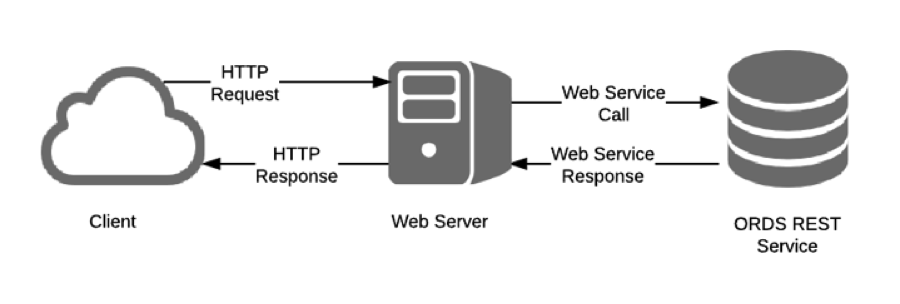
\includegraphics{images/rest.png}

In this section, we will be writing a small Python script to query the Ensembl REST API, a 
database that hosts genomic information stored at the European Bioinformatics Institute.  We 
will search for the reference genome for the bacteriophage \textbf{Escherichia phage ECBP5}, 
information for which can be found \href{https://www.ebi.ac.uk/ena/data/view/KJ749827}{here}.  
The \textbf{accession number} for this genome is KJ749827; accession numbers are an agreed-upon 
unique identifier for a specific biological sequence.  Accession numbers often differ in format 
depending on the database you're working with, so make sure if you're download many genomes that 
the accession numbers are of the correct format for the database you're searching.  \par

To get started, we first need to import the \textbf{requests} module and any other modules that 
we might use.  Then, we will write two functions: one to \textbf{retrieve the sequence of interest} and 
one to \textbf{write the sequence data to a file}.  Here is the full script with a detailed 
explanation below:

\pagebreak
\textbf{query.py}
\vspace{3mm}
\begin{lstlisting}

\end{lstlisting}
\vspace{3mm}

\pagebreak
\subsection{Parsing JSON data}

\pagebreak
\subsection{Regular Expressions}

\pagebreak
\subsection{Interfacing with Bioinformatics Public Resources}

\pagebreak
\subsection{Version Control and GitHub}

\pagebreak
\section{Object Oriented Programming}
\subsection{Python as Objects: What is an Object?}

\pagebreak
\subsection{Classes}

\pagebreak
\subsection{Namespaces}

\pagebreak
\subsection{Modules}

\pagebreak
\section{Computer Science Fundamentals}
\subsection{How Code Interfaces with your Machine}

\pagebreak
\subsection{Computational Cost}

\pagebreak
\subsection{Algorithm Fundamentals}

\pagebreak
\section{Project Design}

\pagebreak
\section{Code Reference}
\subsection{String Operations}

\subsection{List Operations}

\subsection{Array/Tuple Operations}

\subsection{Dictionary Operations}

\subsection{Set Operations}

\subsection{Input/Output}

\subsection{Iterators/Generators}

\subsection{Zip/Map/Reduce}

\subsection{Regular Expressions}





\end{document}









